\chapter{SaltStack}
\label{chap:chapSalt}

This data coming from the minion (e.g., operating system) is called
grains. But there is another type of data: pillar data. While grains
are advertised by the minion back to the master, pillar data is stored
on the master and is made available to each minion individually; that
is, a minion cannot see any pillar data but its own. It is common for
people new to Salt to ask about grains versus pillar data, so we will
discuss them further in Chapter 5. For the moment, you can think of
grains as metadata about the host (e.g., number of CPUs), while pillar
is data the host needs (e.g., a database password). In other words, a
minion tells the master what its grains are, while the minion asks the
master for its pillar data. For now, just know that you can use either
to define the target for a command.

\section{初识SaltStack}
\label{sec:basicSalt}

\begin{figure}[!htbp]
  \centering
  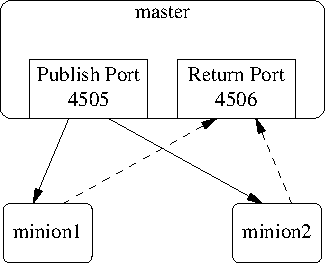
\includegraphics{graph/saltstack_communication.pdf}
  \caption{salt通信示意图}
  \label{fig:saltRelition}
\end{figure}

\section{安装及运行SaltStack}
\label{sec:installSalt}

\subsection{环境准备}
\label{sec:saltEnvPrepare}

以下测试是在CentOS6U5 64位系统上进行测试。系统均关闭iptables及selinux,
如果要开启iptables,请设置允许开放本机的53端口。

\begin{table}[htbp]
  \centering
    \caption{SaltStack测试环境机器列表}
    \label{tab:saltTestMachineList}
    \begin{tabular}{llr}
      \toprule
      主机名     & IP地址 & 说明 \\
      \midrule
      master01.lavenliu.com  & 192.168.20.134 &  Salt Master \\
      minion01.lavenliu.com  & 192.168.20.135 &  Salt Minion \\
      minion02.lavenliu.com  & 192.168.20.136 &  Salt Minion \\
      \bottomrule
    \end{tabular}
\end{table}

假设已经做了DNS解析,如果没有做DNS解析,请在/etc/hosts文件里设置静态主机名解析。
这里使用DNS的方式进行主机名的解析工作,解析测试如下:

\begin{verbatim}
[root@master01 ~]# nslookup master01.lavenliu.com
Server:		192.168.20.134
Address:	192.168.20.134#53

Name:	master01.lavenliu.com
Address: 192.168.20.134

[root@master01 ~]# nslookup minion01.lavenliu.com
Server:		192.168.20.134
Address:	192.168.20.134#53

Name:	minion01.lavenliu.com
Address: 192.168.20.135

[root@master01 ~]# nslookup minion02.lavenliu.com
Server:		192.168.20.134
Address:	192.168.20.134#53

Name:	minion02.lavenliu.com
Address: 192.168.20.136
\end{verbatim}

\subsection{安装SaltStack Master}
\label{sec:installSaltMaster}

使用yum进行salt-master的安装,

\begin{verbatim}
[root@master01 ~]# yum install -y salt-master
\end{verbatim}

将salt-master加入开机自启动,

\begin{verbatim}
[root@master01 ~]# chkconfig salt-master on
\end{verbatim}

\subsection{安装SaltStack Minion}
\label{sec:installSaltMinion}

使用yum进行salt-minion的安装,在minion01及minion02两台机器上进行操作,

\begin{verbatim}
# yum install -y salt-minion
\end{verbatim}

将salt-minion加入开机自启动,在minion01及minion02两台机器上进行操作,

\begin{verbatim}
# chkconfig salt-minion on
\end{verbatim}

\section{SaltStack配置}
\label{sec:saltConfigure}

\subsection{Master端配置}
\label{sec:masterConfigure}

\subsection{Minion端配置}
\label{sec:minionConfigure}

\section{基本使用}
\label{sec:basicUsage}

\subsection{单master设置}
\label{sec:singleMasterSetup}

\subsection{基本命令}
\label{sec:basicSaltCommand}

\subsection{密钥管理}
\label{sec:saltKeyManagement}

\subsection{定位minions}
\label{sec:minionTargeting}

当我们有成千上万台机器时,这些机器承担着不同的角色。有的是HTTP服务器,
有的是DB服务器,有的是文件共享服务器。而且它们分别运行不同的操作系统,
比如,HTTP服务器运行在CentOS系统之上;DB服务器运行在SUSE系统之上;文件
共享服务器运行在FreeBSD系统之上。当我们想在所有的服务器上增加work账号
时,那将是很简单的一件事情。如果WEB服务器只安装httpd,DB服务器只安装
MySQL,文件共享服务器只安装NFS等,如何操作呢?Salt提供了多种选项来帮助
我们定位minions。

\subsubsection*{Minion ID}

最简单的方式就是通过指定具体的minion ID来定位目标机器。如,

\begin{verbatim}
# salt automatic01 test.ping
automatic01:
    True
\end{verbatim}

\subsubsection*{List(-L)选项}

另外,我们可以使用salt命令的\verb|-L|选项,向salt提供一组Minion ID的列
表,如,

\begin{verbatim}
# salt -L mha-manager,automatic01 test.ping
mha-manager:
    True
automatic01:
    True
\end{verbatim}

\subsubsection*{通配符\*}

我们还可以shell-style的通配符,通配符被替换成一组已签过名的minions。\*
表示所有已签名的minions。如,

\begin{verbatim}
# salt '*' test.ping
windows01:
    True
mha-manager:
    True
automatic01:
    True
debian:
    True
\end{verbatim}

通过输出结果,可以看出,这些minions并不是按列表顺序返回的,而是按谁先
返回数据的顺序返回的。

我们还可以使用通配符并结合minions ID一起使用,如,

\begin{verbatim}
# salt 'auto*' test.ping
automatic01:
    True
\end{verbatim}

\subsubsection*{Regular Expression(-E)}

我们可以使用正则表达式来匹配更精确的minions,如,

\begin{verbatim}
# salt -E '.*01' test.ping
windows01:
    True
automatic01:
    True
\end{verbatim}

\subsubsection*{Grains(-G)}

Grains是一组关于操作系统的信息,是在minions启动时加载的,是静态的数据。
Grains提供了操作系统名称和操作系统版本号等。我们可以基于此,只在
CenOS6.5的机器上安装httpd软件包。

如何使用呢?如,

\begin{verbatim}
# salt -G 'os:CentOS' test.ping
automatic01:
    True
mha-manager:
    True
\end{verbatim}

\subsubsection*{Compound(-C)}

接下来的这种方式更为强大一些。它允许我们以组合的形式来匹配minioins。接
下来看一个简单的例子,如,

\begin{verbatim}
# salt -C 'auto* or G@os:Debian' test.ping
automatic01:
    True
debian:
    True

# salt -C 'auto* or L@debian,windows01' test.ping
windows01:
    True
automatic01:
    True
debian:
    True
\end{verbatim}

\section{理解YAML}
\label{sec:understandYAML}

SLS文件的默认渲染器是YAML渲染器。书写SLS文件只有简单的三条规则。

\section{SaltStack配置管理实例}
\label{sec:saltDeployInstances}

接下来,就实际的运用以上的知识点,写出一些可工作的配置管理规则以进行配置管理。只要我们编排好SLS文件,Salt就会按照我们的编排进行自动的配置管理。

看一下目录结构:

\begin{verbatim}
[root@master01 states]# pwd
/etc/salt/states
[root@master01 states]# tree
.
├── init
│   ├── files
│   │   ├── limits.conf
│   │   └── vimrc
│   ├── pkg.sls
│   ├── test.sls
│   └── vim.sls
├── prod
│   ├── elk
│   │   ├── elasticsearch.sls
│   │   ├── files
│   │   │   ├── elasticsearch-1.7.0.tar.gz
│   │   │   ├── elasticsearch_plugins.tar.gz
│   │   │   ├── elasticsearch.yml
│   │   │   ├── es-service.tar.gz
│   │   │   ├── indexer.conf
│   │   │   ├── kibana-4.1.1-linux-x64.tar.gz
│   │   │   ├── logstash-1.5.3.tar.gz
│   │   │   ├── logstash-2.3.1-1.noarch.rpm
│   │   │   ├── logstash.sh
│   │   │   ├── master.tar.gz
│   │   │   └── shipper.conf
│   │   ├── indexer.sls
│   │   ├── install.sls
│   │   ├── kibana.sls
│   │   ├── logstash.sls
│   │   └── shipper.sls
│   ├── haproxy
│   │   ├── files
│   │   │   ├── haproxy-1.5.15.tar.gz
│   │   │   └── haproxy.init
│   │   └── install.sls
│   ├── jdk
│   │   ├── files
│   │   │   └── jdk-8u65-linux-x64.tar.gz
│   │   └── install.sls
│   ├── keepalived
│   │   └── files
│   │       └── keepalived-1.2.16.tar.gz
│   ├── libevent
│   │   ├── files
│   │   │   └── libevent-2.0.22-stable.tar.gz
│   │   └── install.sls
│   ├── logstash.zip
│   ├── memcached
│   │   ├── files
│   │   │   └── memcached-1.4.25.tar.gz
│   │   ├── install.sls
│   │   └── service.sls
│   ├── mysql
│   │   ├── files
│   │   │   └── mysql-5.5.32.tar.gz
│   │   └── install.sls
│   ├── nginx
│   │   └── files
│   ├── pkg
│   │   └── pkg-init.sls
│   ├── redis
│   │   ├── files
│   │   │   └── redis.conf
│   │   └── server.sls
│   └── tomcat
│       ├── files
│       │   └── apache-tomcat-8.0.28.tar.gz
│       └── install.sls
└── top.sls

27 directories, 76 files
\end{verbatim}

\subsection{安装JDK}
\label{sec:saltInstallJDK}

\begin{verbatim}
[root@master01 states]# cat prod/jdk/install.sls 
jdk-install:
  file.managed:
    - name: /usr/local/src/jdk-8u65-linux-x64.tar.gz
    - source: salt://prod/jdk/files/jdk-8u65-linux-x64.tar.gz
    - user: root
    - group: root
    - mode: 644
  cmd.run:
    - name: cd /usr/local/src && tar -xf jdk-8u65-linux-x64.tar.gz && mv jdk1.8.0_65 jdk && chown -R root:root jdk
    - unless: test -d /usr/local/jdk

/etc/profile:
  file.append:
    - text:
      - export JAVA_HOME=/usr/local/jdk
      - export JRE_HOME=${JAVA_HOME}/jre
      - CLASS_PATH=${JAVA_HOME}/lib:${JRE_HOME}/lib
      - PATH=$PATH:$JAVA_HOME/bin
\end{verbatim}

\subsection{安装Tomcat}
\label{sec:saltInstallTomcat}

\subsection{安装Nginx}
\label{sec:saltInstallNginx}

\subsection{安装MySQL}
\label{saltInstallMySQL}

\subsection{安装PHP}
\label{sec:saltInstallPHP}

\subsection{安装Redis}
\label{sec:saltInstallRedis}

\subsection{安装ELK Stack}
\label{sec:saltInstallELK}

\subsection{安装OpenStack}
\label{sec:saltInstallOpenStack}


%%% Local Variables:
%%% mode: latex
%%% TeX-master: t
%%% End:
